% Development, review and release workflow for a streamPAMI algorithm.
% Compile: pdflatex developmentWorkflowStreamPAMI.tex
\documentclass[tikz,border=8pt]{standalone}
\usetikzlibrary{positioning,arrows.meta,shapes.geometric,shapes.symbols,calc}

\definecolor{devblue}{HTML}{4472C4}
\definecolor{revorange}{HTML}{F4B83F}
\definecolor{relgreen}{HTML}{6AA84F}
\definecolor{lanered}{HTML}{E02020}
\colorlet{devlight}{devblue!45}
\colorlet{revlight}{revorange!60}
\colorlet{rellight}{relgreen!45}
\colorlet{revdark}{revorange!85!black}
\newcommand{\sub}{\footnotesize}

\begin{document}
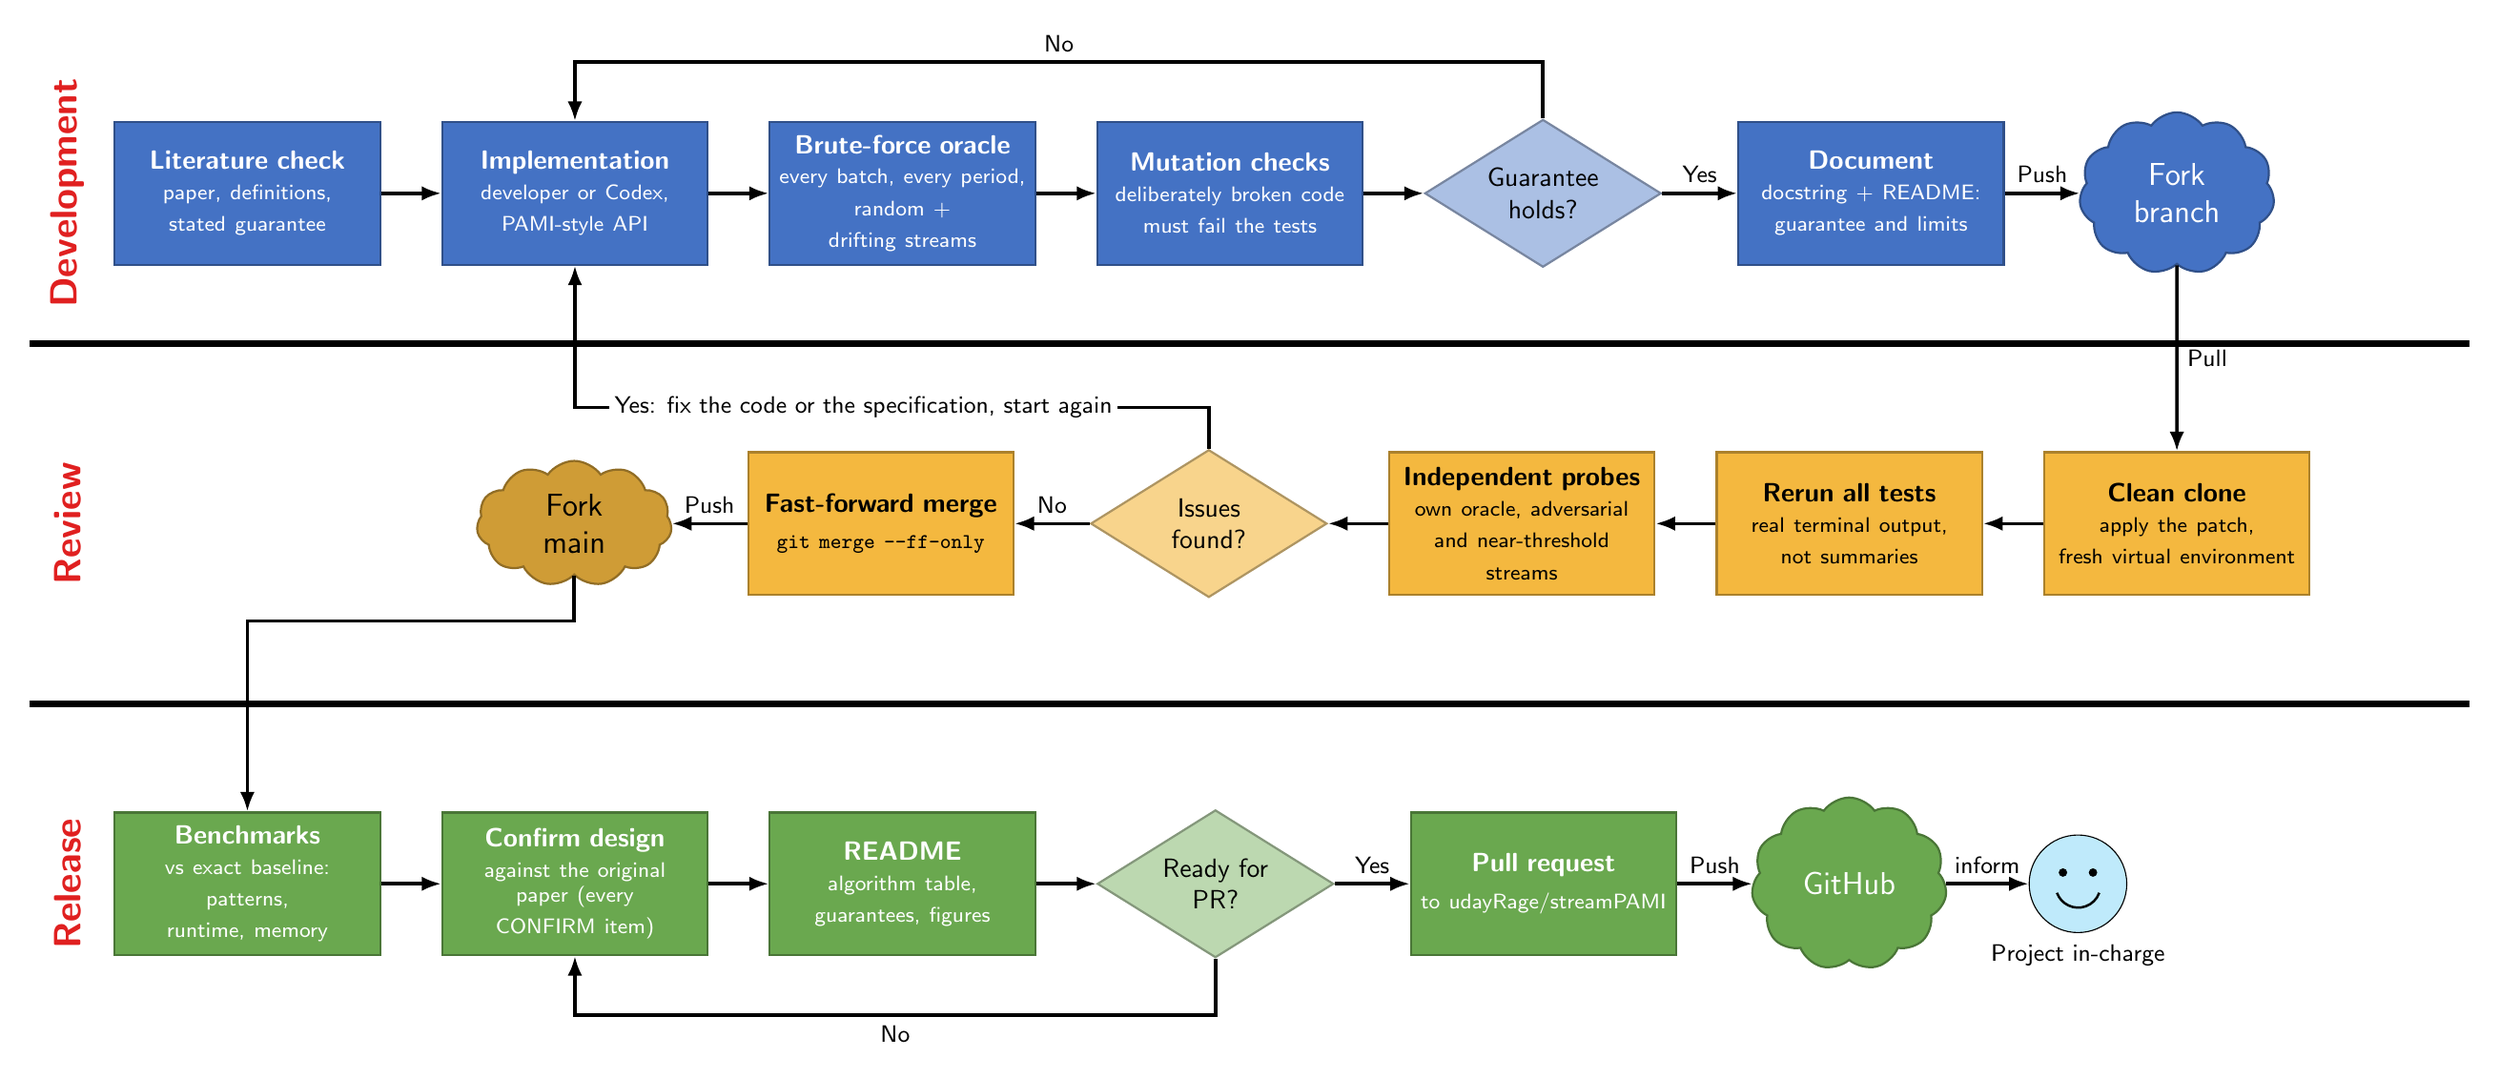
\begin{tikzpicture}[
    font=\sffamily,
    every node/.append style={execute at begin node={\hyphenpenalty=10000\exhyphenpenalty=10000}},
    >={Latex[length=2.6mm]},
    arr/.style={->, line width=1.3pt},
    box/.style={draw=#1!70!black, fill=#1, text=white, minimum width=3.5cm,
                minimum height=1.9cm, align=center, text width=3.3cm, line width=0.8pt},
    dec/.style={diamond, aspect=1.6, draw=#1!70!black, fill=#1, text=black,
                align=center, inner sep=1pt, text width=1.9cm, line width=0.8pt},
    gitcloud/.style={cloud, cloud puffs=11, cloud puff arc=110, draw=#1!70!black, fill=#1,
                  text=white, minimum width=2.6cm, minimum height=1.6cm, align=center,
                  font=\sffamily\large, line width=0.8pt},
    sub/.style={font=\sffamily\footnotesize},
    lane/.style={font=\sffamily\bfseries\Large, text=lanered, rotate=90},
    yes/.style={font=\sffamily\small, pos=0.3},
]

% ======================= Development =======================
\node[lane] at (-2.4, 0) {Development};
\node[box=devblue] (lit) at (0,0)
  {\textbf{Literature check}\\[2pt]\sub paper, definitions,\\stated guarantee};
\node[box=devblue, right=0.8cm of lit] (impl)
  {\textbf{Implementation}\\[2pt]\sub developer or Codex,\\PAMI-style API};
\node[box=devblue, right=0.8cm of impl] (oracle)
  {\textbf{Brute-force oracle}\\[2pt]\sub every batch, every period,\\random + drifting streams};
\node[box=devblue, right=0.8cm of oracle] (mut)
  {\textbf{Mutation checks}\\[2pt]\sub deliberately broken code\\must fail the tests};
\node[dec=devlight, right=0.8cm of mut] (ok) {Guarantee\\holds?};
\node[box=devblue, right=1.0cm of ok] (doc)
  {\textbf{Document}\\[2pt]\sub docstring + README:\\guarantee and limits};
\node[gitcloud=devblue, right=1.0cm of doc] (fork) {Fork\\branch};

\draw[arr] (lit) -- (impl);
\draw[arr] (impl) -- (oracle);
\draw[arr] (oracle) -- (mut);
\draw[arr] (mut) -- (ok);
\draw[arr] (ok) -- node[above, font=\sffamily\small] {Yes} (doc);
\draw[arr] (doc) -- node[above, font=\sffamily\small] {Push} (fork);
\draw[arr] (ok.north) -- ++(0,0.75) -| node[pos=0.25, above, font=\sffamily\small] {No} (impl.north);

% separator
\draw[line width=2.5pt] (-2.9,-2.0) -- (29.6,-2.0);

% ======================= Review =======================
\node[lane] at (-2.4, -4.4) {Review};
\coordinate (reviewrow) at (0,-4.4);
\node[box=revorange, text=black] (clean) at (fork |- reviewrow)
  {\textbf{Clean clone}\\[2pt]\sub apply the patch,\\fresh virtual environment};
\node[box=revorange, text=black, left=0.8cm of clean] (rerun)
  {\textbf{Rerun all tests}\\[2pt]\sub real terminal output,\\not summaries};
\node[box=revorange, text=black, left=0.8cm of rerun] (probe)
  {\textbf{Independent probes}\\[2pt]\sub own oracle, adversarial\\and near-threshold streams};
\node[dec=revlight, left=0.8cm of probe] (issue) {Issues\\found?};
\node[box=revorange, text=black, left=1.0cm of issue] (merge)
  {\textbf{Fast-forward merge}\\[2pt]\sub \texttt{git merge --ff-only}};
\node[gitcloud=revdark, text=black, left=1.0cm of merge] (main) {Fork\\main};

\draw[arr] (fork.south) -- node[right, font=\sffamily\small] {Pull} (clean.north);
\draw[arr] (clean) -- (rerun);
\draw[arr] (rerun) -- (probe);
\draw[arr] (probe) -- (issue);
\draw[arr] (issue) -- node[above, font=\sffamily\small] {No} (merge);
\draw[arr] (merge) -- node[above, font=\sffamily\small] {Push} (main);
\draw[arr] (issue.north) -- ++(0,0.55) -| (impl.south);
\node[font=\sffamily\small, fill=white, inner sep=2pt] at ($(issue.north)+(-4.6,0.55)$)
   {Yes: fix the code or the specification, start again};

% separator
\draw[line width=2.5pt] (-2.9,-6.8) -- (29.6,-6.8);

% ======================= Release =======================
\node[lane] at (-2.4, -9.2) {Release};
\node[box=relgreen] (bench) at (0,-9.2)
  {\textbf{Benchmarks}\\[2pt]\sub vs exact baseline:\\patterns, runtime, memory};
\node[box=relgreen, right=0.8cm of bench] (paper)
  {\textbf{Confirm design}\\[2pt]\sub against the original\\paper (every\\CONFIRM item)};
\node[box=relgreen, right=0.8cm of paper] (readme)
  {\textbf{README}\\[2pt]\sub algorithm table,\\guarantees, figures};
\node[dec=rellight, right=0.8cm of readme] (ready) {Ready for\\PR?};
\node[box=relgreen, right=1.0cm of ready] (pr)
  {\textbf{Pull request}\\[2pt]\sub to udayRage/streamPAMI};
\node[gitcloud=relgreen, right=1.0cm of pr] (up) {GitHub};
\node[circle, draw=black, fill=cyan!25, minimum size=1.3cm, right=1.1cm of up] (pic) {};
\fill (pic.center) ++(-0.2,0.15) circle (1.6pt) ++(0.4,0) circle (1.6pt);
\draw[line width=0.9pt] (pic.center) ++(-0.28,-0.12) arc[start angle=200, end angle=340, radius=0.3];
\node[below=1pt of pic, font=\sffamily\small] {Project in-charge};

\draw[arr] (main.south) -- ++(0,-0.6) -| (bench.north);
\draw[arr] (bench) -- (paper);
\draw[arr] (paper) -- (readme);
\draw[arr] (readme) -- (ready);
\draw[arr] (ready) -- node[above, font=\sffamily\small] {Yes} (pr);
\draw[arr] (pr) -- node[above, font=\sffamily\small] {Push} (up);
\draw[arr] (up) -- node[above, font=\sffamily\small] {inform} (pic);
\draw[arr] (ready.south) -- ++(0,-0.75) -| node[pos=0.25, below, font=\sffamily\small] {No} (paper.south);
\end{tikzpicture}
\end{document}
